\subsection{\bf Flow Duration Analysis}
The flow duration distributions for each kind of workloads are shown in figure \ref{fig:read_duration}, \ref{fig:write_duration} and \ref{fig:replica_duration}.

\begin{figure*}[!htpb]
\label{fig:read_duration}
\centering
  \begin{subfigure}[b]{.45\linewidth}
   \centering
	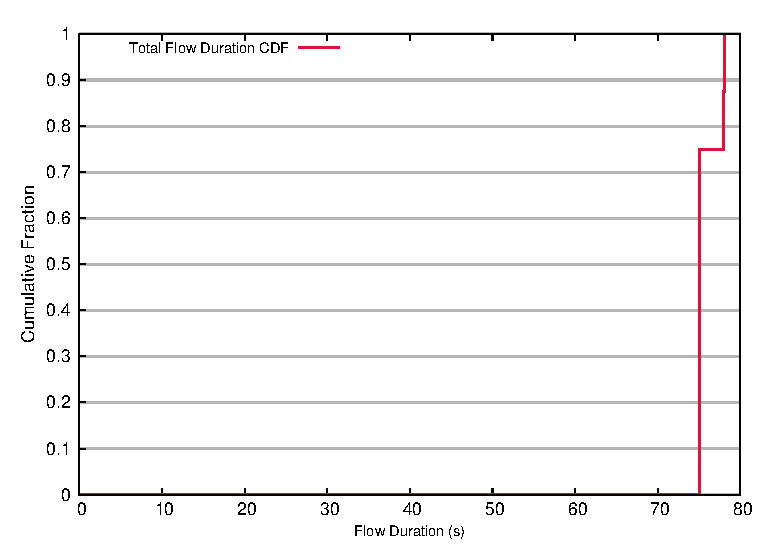
\includegraphics[width=.99\textwidth]{figures/4read/24_28_flow_duration.eps} 
	\caption{RPC between Client and DataNodes}\label{fig:read_duration:rpc}
   \end{subfigure}%
  \begin{subfigure}[b]{.45\linewidth}
   \centering
	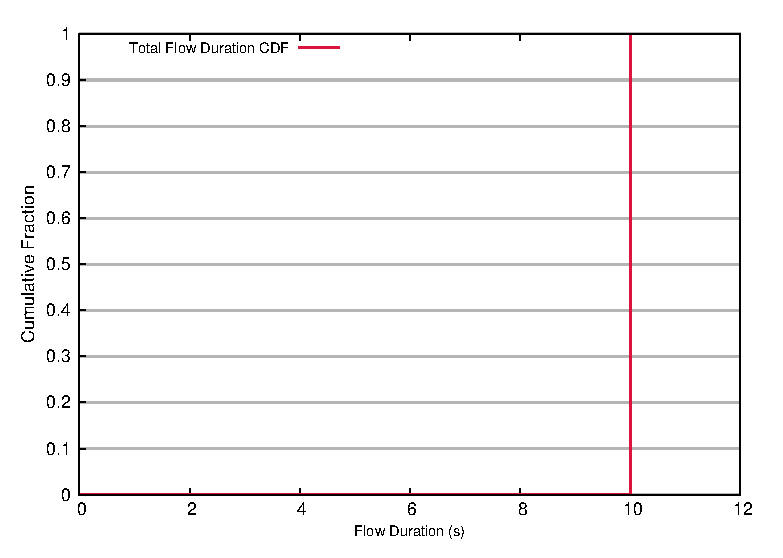
\includegraphics[width=.99\textwidth]{figures/4read/8_12_flow_duration.eps} 
	\caption{Should have read data transfer here}\label{fig:read_duration:fixme}
   \end{subfigure} \\%
  \begin{subfigure}[b]{.55\linewidth}
   \centering
	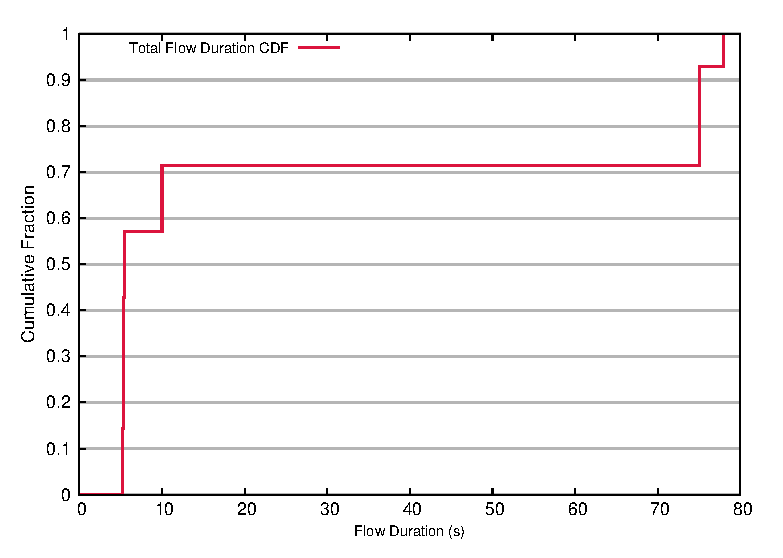
\includegraphics[width=.99\textwidth]{figures/4read/flow_duration.eps}
	\caption{All Traffic}\label{fig:read_duration:all}
   \end{subfigure}%
\caption{Read Flow Duration Distribution}
\end{figure*}

FXIME: read workload doesn't make sense here, needs to fix it.


\begin{figure*}[!htbp]
\label{fig:write_duration}
\centering
  \begin{subfigure}[b]{.45\linewidth}
   \centering
	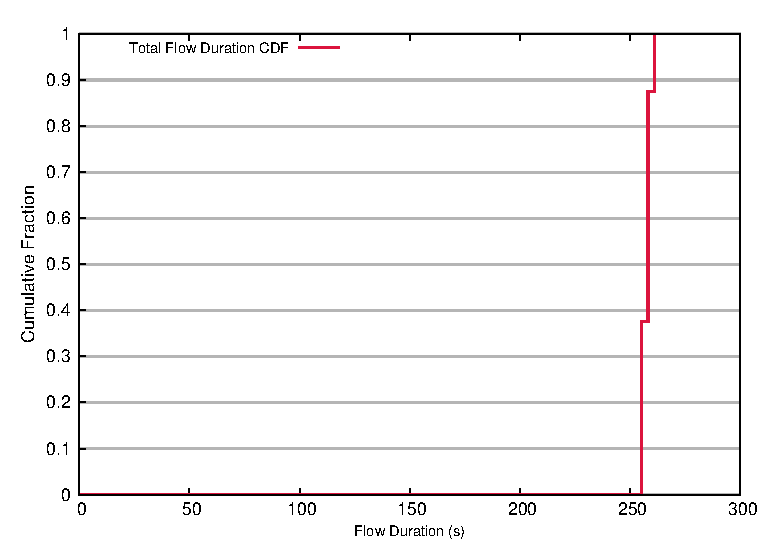
\includegraphics[width=.99\textwidth]{figures/6writes/24_28_type_flow_duration.eps} 
	\caption{DataNodes RPC with NameNode}\label{fig:write_duration:dn_rpc}
   \end{subfigure}%
  \begin{subfigure}[b]{.45\linewidth}
   \centering
	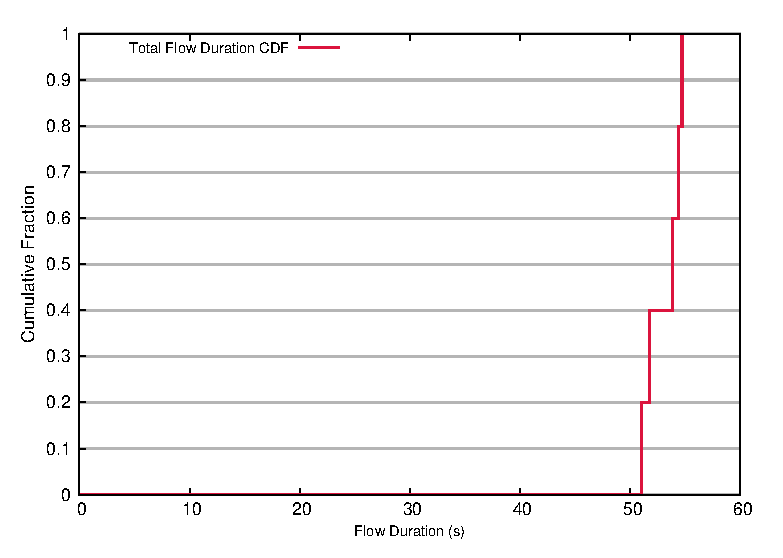
\includegraphics[width=.99\textwidth]{figures/6writes/24_28_20_16_type_flow_duration.eps} 
	\caption{Client and DataNodes RPC with NameNode}\label{fig:write_duration:dc_rpc}
   \end{subfigure} \\%
  \begin{subfigure}[b]{.45\linewidth}
   \centering
	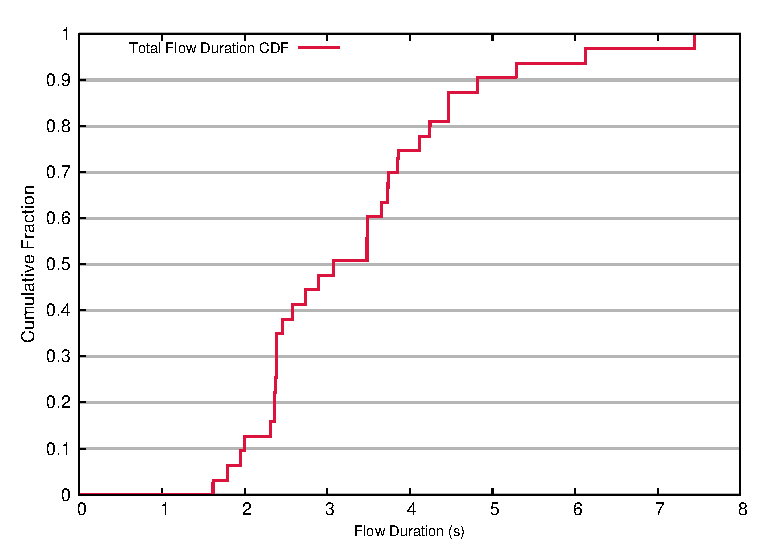
\includegraphics[width=.99\textwidth]{figures/6writes/36_44_type_flow_duration.eps} 
	\caption{Pipelined Writes between DataNodes}\label{fig:write_duration:pipe_write}
   \end{subfigure} %
  \begin{subfigure}[b]{.45\linewidth}
   \centering
	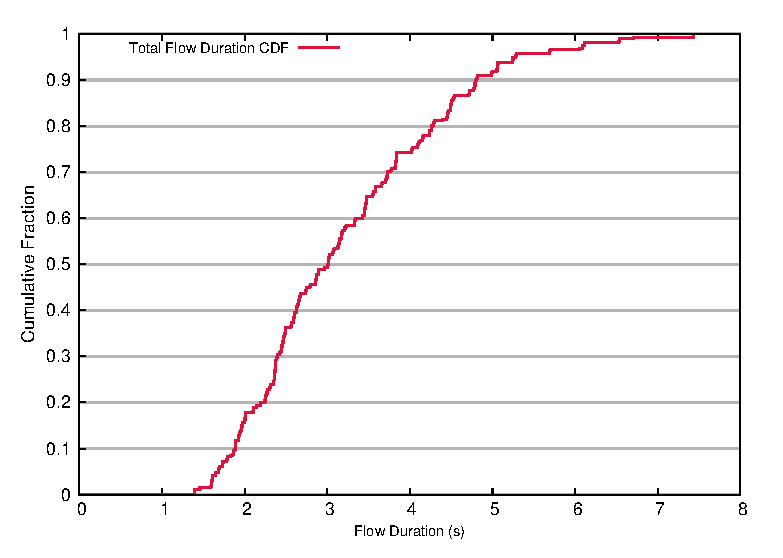
\includegraphics[width=.99\textwidth]{figures/6writes/32_36_type_flow_duration.eps} 
	\caption{Client Data Transfer to DataNodes}\label{fig:write_duration:client_write}
   \end{subfigure} \\%
  \begin{subfigure}[b]{.45\linewidth}
   \centering
	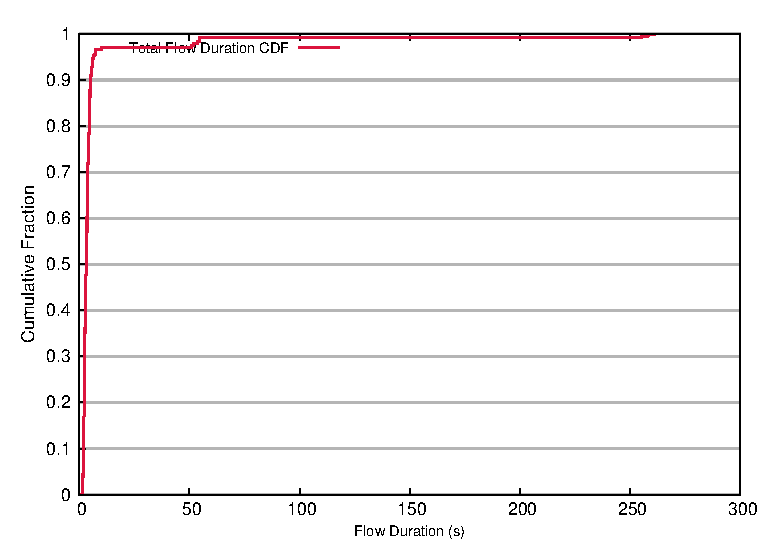
\includegraphics[width=.99\textwidth]{figures/6writes/flow_duration.eps}
	\caption{All Traffic}\label{fig:write_duration:all}
   \end{subfigure}%
  \begin{subfigure}[b]{.45\linewidth}
   \centering
	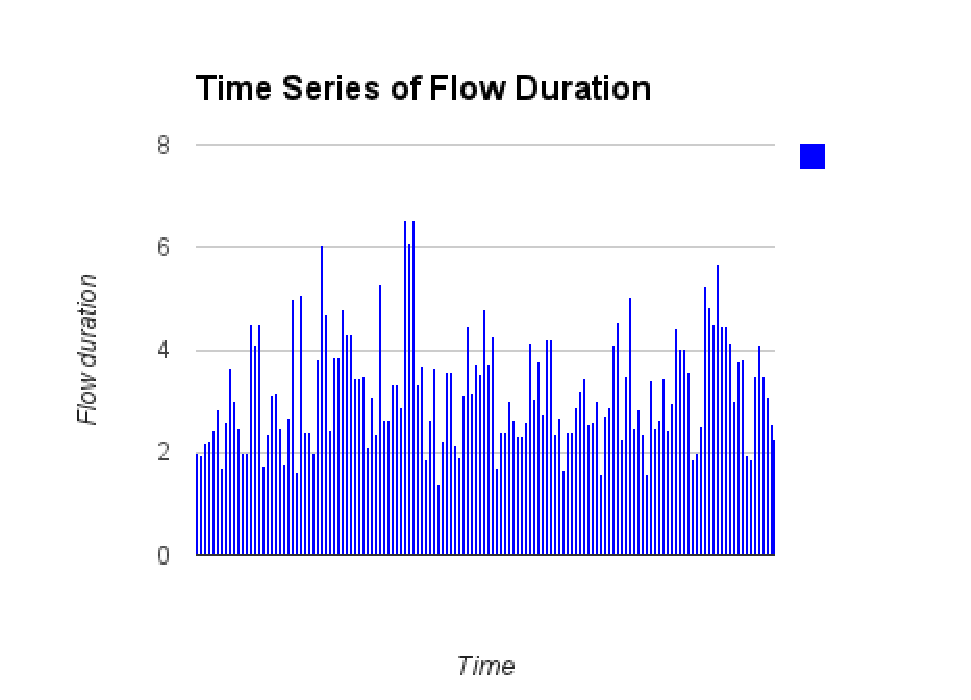
\includegraphics[width=.99\textwidth]{figures/6writes/flow_duration_time_series.eps}
	\caption{Time Series of All Traffic}\label{fig:write:time_series}
   \end{subfigure}%
\caption{Write Flow Duration Distribution}
\end{figure*}

For the write workload, we can again see the radical differences between RPC calls/responds flows, which are long lived and shared amoung multiple RPC calls; and data transfer flows, which transfers one block of file data in HDFS in its lifetime. However, we have noticed that the data transfer flows' duration spans a wide range, from less than 2 seconds to more than seven seconds, even though all of them transfer the same amount of data. In order to determine whether this is caused by network congestion or any hotspots within the network, we looked the flow duration on each link of the network, and found that this distribution is not dependent on the network location. Actually flows between any two nodes in our network exhibit the similar duration distribution (results omitted in the interest of space). The time series of the flow duration is also shown in figure \ref{fig:write:time_series}, and we could see periodic spike in the flow duration. We think it could be related to the network condition, but no further information is avaiable to investigate the cause of it.

\begin{figure*}[!htbp]
\label{fig:replica_duration}
\centering
  \begin{subfigure}[b]{.45\linewidth}
   \centering
	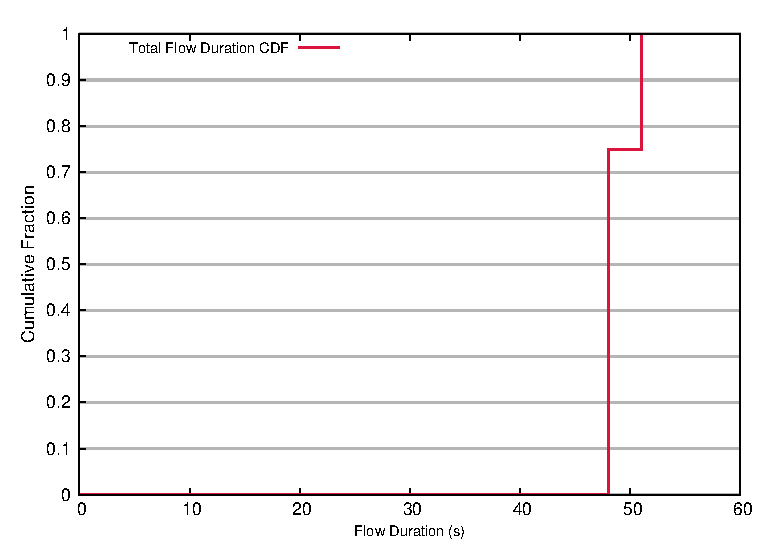
\includegraphics[width=.99\textwidth]{figures/replica_change/24_28_flow_duration.eps} 
	\caption{DataNodes RPC with NameNode}\label{fig:replica_duration:rpc}
   \end{subfigure}%
  \begin{subfigure}[b]{.45\linewidth}
   \centering
	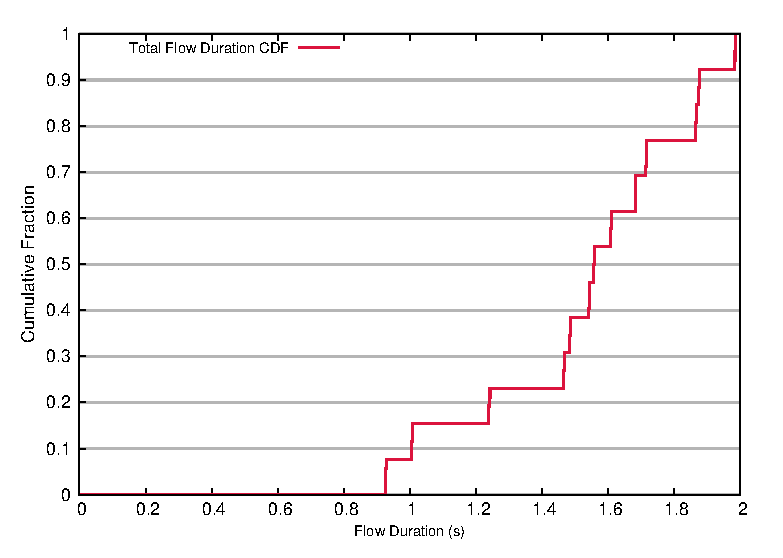
\includegraphics[width=.99\textwidth]{figures/replica_change/36_32_flow_duration.eps} 
	\caption{Pipelined Writes between DataNodes}\label{fig:replica_duration:pipe_write}
   \end{subfigure} \\%
  \begin{subfigure}[b]{.55\linewidth}
   \centering
	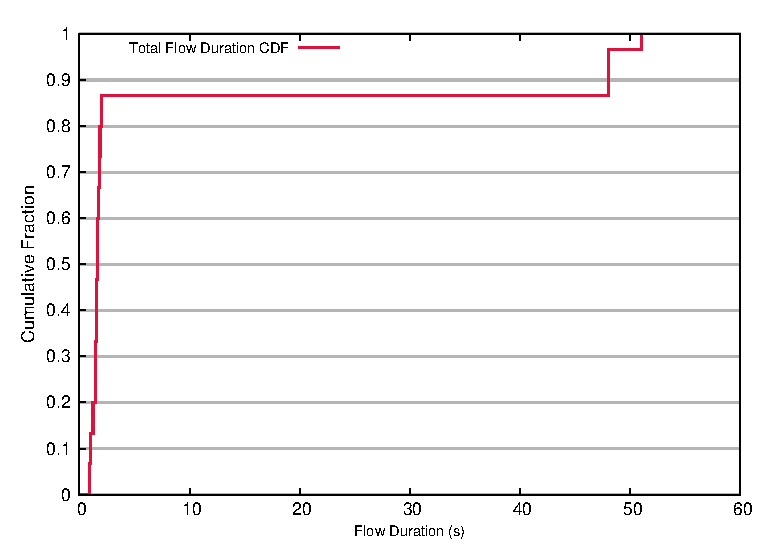
\includegraphics[width=.99\textwidth]{figures/replica_change/flow_duration.eps}
	\caption{All Traffic}\label{fig:read_duration:all}
   \end{subfigure}%
\caption{Replciation Level Change Flow Duration Distribution}
\end{figure*}

The flow duration distribution of the replication level change workload in figure \ref{fig:replica_duration} exihibed the same characteristics, except for that there is fewer data transfered, thus flows are generally shorter. 

